% Charlotte Geiger - Manuel Lippert - Leonard Schatt
% Physikalisches Praktikum

% Teilaufgabe 4

\section{Lage der Achsen bei Nutation eines momentfreien Kreisels}

\begin{figure}
    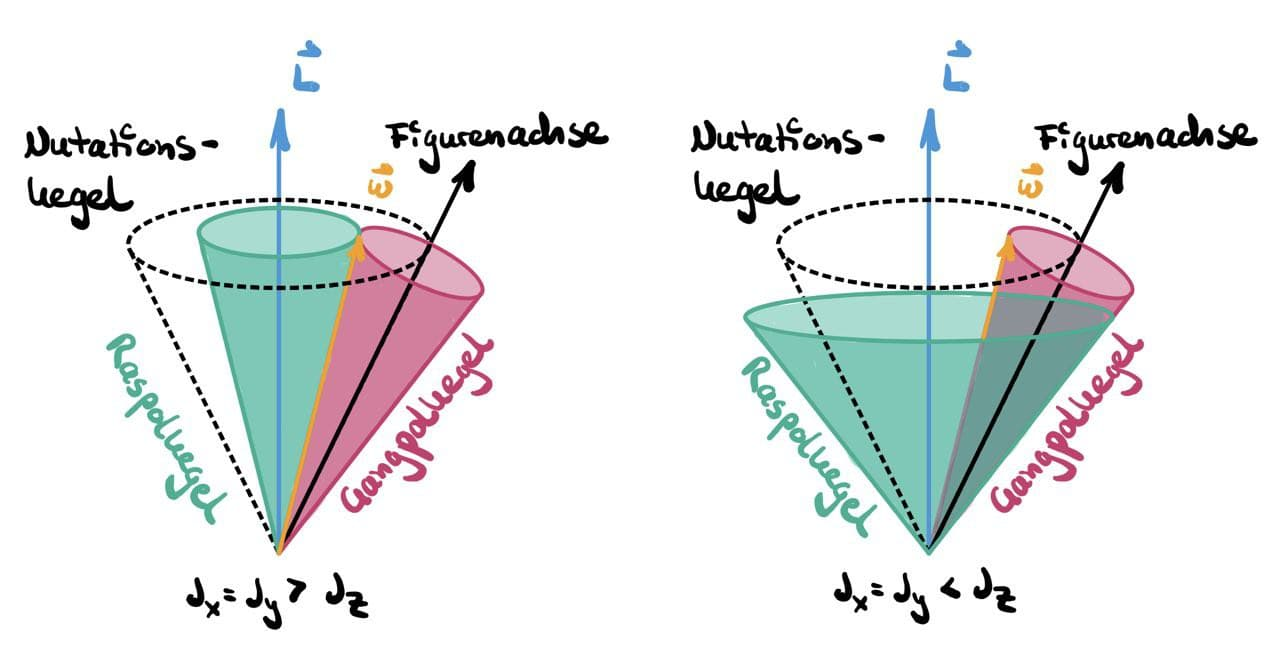
\includegraphics[scale=0.3]{Nutationsbewegung.jpg}
    \captionof{figure}{Nutationsbewegung für unterscheidliche Trägheitsmomente}
\end{figure}

Bei einem momentfreien Kreisel ist die Drehimpulsachse fest im Raum. Diese wird umschlossen von dem sogenannten \dq Raspolkegel\dq{}, welcher auch fest im Raum steht. Die Figurenachse bewegt sich mit der Nutationswinkelgeschwindigkeit $w_n$ um den Nutationskegel. Dabei ist die Figurenachse von dem sogenannten \dq Gangpolkegel\dq{} umschlossen, welcher sich auf dem Raspolkegel \dq abrollt\dq{} und somit den Nutationskegel entstehen lässt. Weiterhin ist die relative Lage des Raspolkegels und des Gangpolkegels zueinander festgelegt durch das Trägheitsmoment bzgl der Drehimpulsachse. % Grafik ref